\documentclass{article}
\usepackage[T2A]{fontenc}
\usepackage[utf8]{inputenc}
\usepackage{graphicx}

\graphicspath{ {./img/} }

\newcommand{\paragraphline}[1]{\paragraph{#1}\mbox{}\\}

\title{Cartesian closed categories and the price of eggs}
\author{Jane Doe}
\date{September 1994}
\begin{document}
    \maketitle
    \section{Актеры}
    \begin{enumerate}
        \item Администратор (Преподаватель) - пользователь, которые имеет права на создание и редактирование тестовых шаблонов, а также может создавать тестовые события и назначать их группам студентов.
        \item Пользователь (Студент или Преподаватель) - пользователь, которые имеет права на прохождение назначенных ему событий и просмотр результатов.
    \end{enumerate}
    
    % \textbf{}

    % \paragraph{Создать/Редактировать тестовый шаблон}
    \section{Варианты использования}
    \paragraphline{Создать/Редактировать тестовый шаблон}
    \textbf{Описание:} Администратор изменяет существующий тестовый шаблон\\
    \textbf{Предусловия:}Тестовый шаблон создан\\
    \textbf{Основной поток событий:}
    \begin{enumerate}
        \item Администратор открывает страницу создания/редактирования шаблона
        \item Администратор изменяет имя шаблона
        \item Если Администратор желает Добавить/Редактировать тестовый вопрос, выполняется вариант использования Добавить/Редактировать тестовый вопрос.
        \item Если Администратор желает удалить тестовый вопрос, выполняется вариант использования Удалить вопрос.
        \item Вариант использования завершается
        \item Администратор сохраняет шаблон
    \end{enumerate} 
    
    \paragraphline{Добавить тестовый вопрос}
    \textbf{Описание:} Администратор добавляет новый вопрос в тестовый шаблон\\
    \textbf{Предусловия:} Тестовый шаблон создан\\
    \textbf{Основной поток событий:}
    \begin{enumerate}
        \item Администратор добавляет пустой тестовый вопрос
        \item Администратор задает текст вопроса
        \item Если Администратор желает задать сигнатуру тестовой процедуры, выполняется вариант использования Задать вид тестовой процедуры.
        \item Если Администратор желает добавить верное решение решение в виде процедуры, выполняется вариант использования Задать верное решение.
        \item Если Администратор желает задать набор входных тестовых данных , выполняется вариант использования Задать входные данные для тестирования
        \item Вариант использования завершается
    \end{enumerate}


    \paragraphline{Задать вид тестовой процедуры}
    \textbf{Описание:} Администратор создает объект процедуры, описывающей вид входных и выходных данных\\
    \textbf{Предусловия:} Тестовый вопрос создан\\
    \textbf{Основной поток событий:}
    \begin{enumerate}
        \item Администратор задает название процедуры в соответствующем поле
        \item Администратор выбирает тип возвращаемого процедурой значения из списка допустимых значений.
        \item Администратор задает набор входных параметров
        \item Вариант использования завершается
        \item Задать верное решение
    \end{enumerate}
    
    \paragraphline{Задать верное решение}
    \textbf{Описание:} Администратор задает код процедуры, который решает поставленную в вопросе задачу и выдает результаты, с которыми впоследствии будут сравниваться результаты, полученные от пользовательского кода\\
    \textbf{Предусловия:} Тестовый процедура создана\\
    \textbf{Основной поток событий:}
    \begin{enumerate}
        \item Администратор записывает код процедуры в соответствующем поле
        \item Вариант использования завершается
    \end{enumerate}

    \paragraphline{Задать входные данные для тестирования}
    \textbf{Описание:} Администратор задает наборы значений всех входных аргументов для тестируемой функции\\
    \textbf{Предусловия:} Тестовый процедура создана\\
    \textbf{Основной поток событий:}
    \begin{enumerate}
        \item Администратор записывает наборы входных данных в определенном в формате в соответствующее поле
        \item Вариант использования завершается
    \end{enumerate}
    
    \paragraphline{Просмотреть список шаблонов}
    \textbf{Описание:} Администратор просматривает список существующих тестовых шаблонов, доступных для редактирования или создания события\\
    \textbf{Предусловия:} Нет\\
    \textbf{Основной поток событий:}
    \begin{enumerate}
        \item Администратор записывает наборы входных данных в определенном в формате в соответствующее поле
        \item Вариант использования завершается
    \end{enumerate}

    
    \paragraphline{Создать тестовое событие}
    \textbf{Описание:} Администратор создает тестовое событие на основе одного из шаблонов и задает список студентов, которые должны пройти это событие.
    \textbf{Предусловия:} Существует хотя бы один тестовый шаблон
    \textbf{Основной поток событий:}
    \begin{enumerate}
        \item Если Администратор желает задать время начала/окончания события, выполняется вариант использования Задать дату и время начала/окончания события.
        \item Если Администратор желает выбрать тестовый шаблон для события, выполняется вариант использования Выбрать тестовый шаблон.
        \item Если Администратор желает задать список студентов, которым необходимо пройти тестовое событие, выполняется вариант использования Указать список тестируемых студентов
        \item Администратор нажимает кнопку “Создать”
        \item Вариант использования завершается
    \end{enumerate}



    \paragraphline{Задать дату и время начала/окончания события}
    \textbf{Описание:} Администратор задает временной промежуток, в течение которого пользователям будет доступно это событие.
    \textbf{Предусловия:} Выполняется вариант использования Создать тестовое событие
    \textbf{Основной поток событий:}
    \begin{enumerate}
        \item Администратор выбирает дату и время начала и окончания события на интерфейсе
        \item Вариант использования завершается
    \end{enumerate}

    \paragraphline{Выбрать тестовый шаблон}
    \textbf{Описание:} Администратор выбирает один из существующих тестовых шаблонов, который будет использован при проведении события
    \textbf{Предусловия:} 
    \begin{enumerate}
       \item Существует хотя бы один тестовый шаблон
       \item Выполняется вариант использования “Создать тестовое событие”
    \end{enumerate}

    \textbf{Основной поток событий:}
    \begin{enumerate}
        \item Администратор выбирает тестовый шаблон из предоставленного списка
        \item Администратор нажимает кнопку “Подтвердить”
        \item Вариант использования завершается    
    \end{enumerate}

    \paragraphline{Указать список тестируемых студентов}
    \textbf{Описание:} Администратор выбирает студентов, которым необходимо пройти это тестовое событие\\
    \textbf{Предусловия:} Выполняется вариант использования “Создать тестовое событие”
    \textbf{Основной поток событий:}
    \begin{enumerate}
        \item Администратор выбирает студентов/группы студентов из списка
        \item Вариант использования завершается
    \end{enumerate}

    \paragraphline{Просмотреть список доступных тестовых событий}
    \textbf{Описание:} Пользователь просматривает список событий, которые были на него назначены\\
    \textbf{Предусловия:} Нет\\
    \textbf{Основной поток событий:}
    \begin{enumerate}
        \item Пользователь открывает страницу со списком доступных событий
        \item Вариант использования завершается
    \end{enumerate}

    \paragraphline{Запустить тестовое событие}
    \textbf{Описание:} Пользователь начинает одно из назначенных ему тестовых событий\\
    \textbf{Предусловия:} 
    \begin{enumerate}
        \item Пользователь имеет назначенные на него события
        \item Событие уже стало доступно и еще не закончилось
    \end{enumerate}
    
    \textbf{Основной поток событий:}
    \begin{enumerate}
        \item Пользователь выбирает событие и нажимает кнопку “Начать”.
        \item Пользователь вводит ответы на вопросы теста.
        \item Если пользователь желает проверить правильность своего решения, выполняется вариант использования Запросить проверку решения.
        \item Пользователь нажимает кнопку “Завершить”
        \item Вариант использования завершается    
    \end{enumerate}

    \paragraphline{Запросить проверку решения}
    \textbf{Описание:} Пользователь запрашивает проверку своего решения для вопроса\\
    \textbf{Предусловия:} Выполняется вариант использования “Запустить тестовое событие”\\
    \textbf{Основной поток событий:}
    \begin{enumerate}
        \item Пользователь нажимает кнопку “Проверить решение” и через некоторое время получает результат проверки
        \item Вариант использования завершается
    \end{enumerate}

    \paragraphline{Просмотреть результаты пройденных тестов}
    \textbf{Описание:} Пользователь просматривает историю своих пройденных событий\\
    \textbf{Предусловия:} Нет\\
    \textbf{Основной поток событий:}
    \begin{enumerate}
        \item Пользователь переходит на страницу с результатами пройденных тестов
        \item Вариант использования завершается
    \end{enumerate}

    \section{Диаграммы классов}
    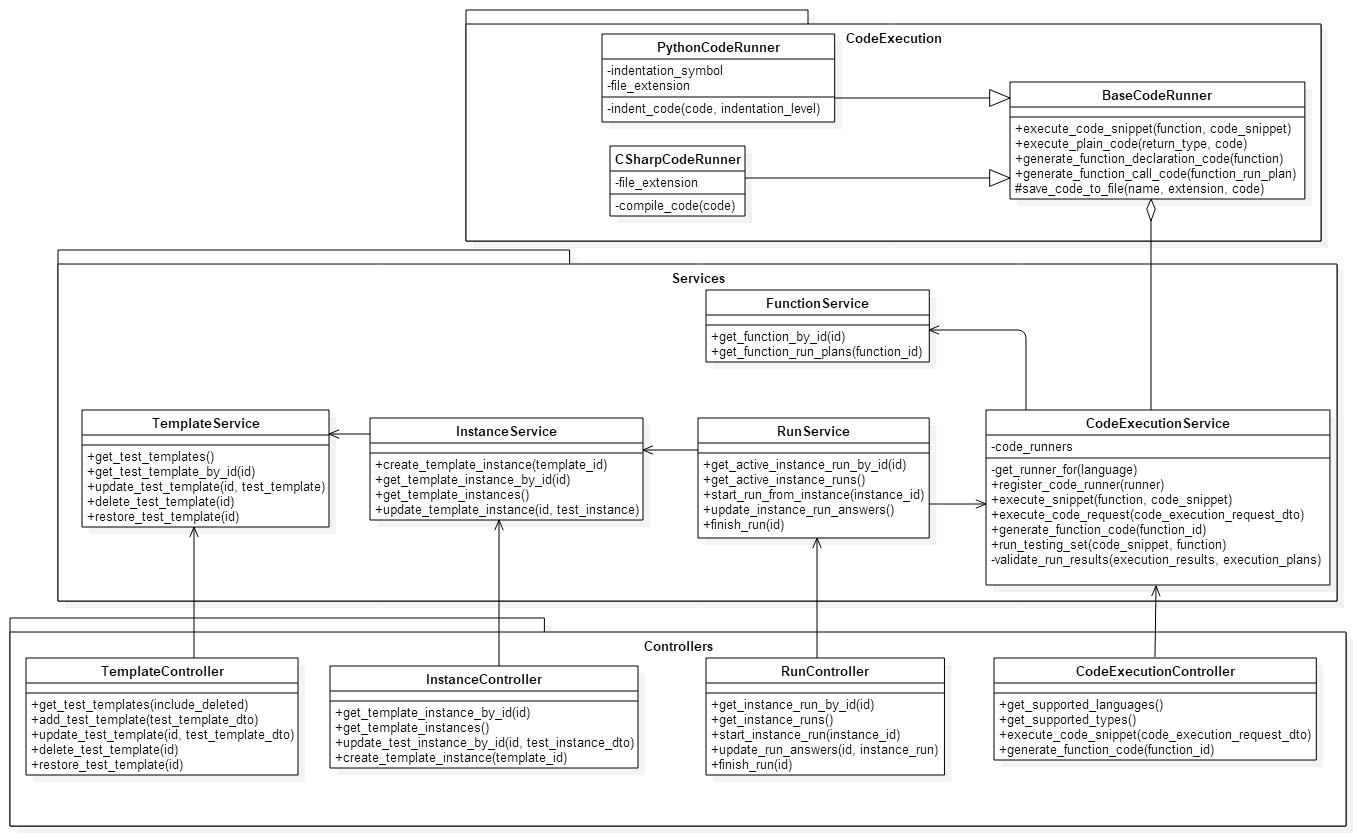
\includegraphics[width=\textwidth,height=\textheight,keepaspectratio,angle=270]{ClassDiagram_Services}
    test
    \pagebreak
    % 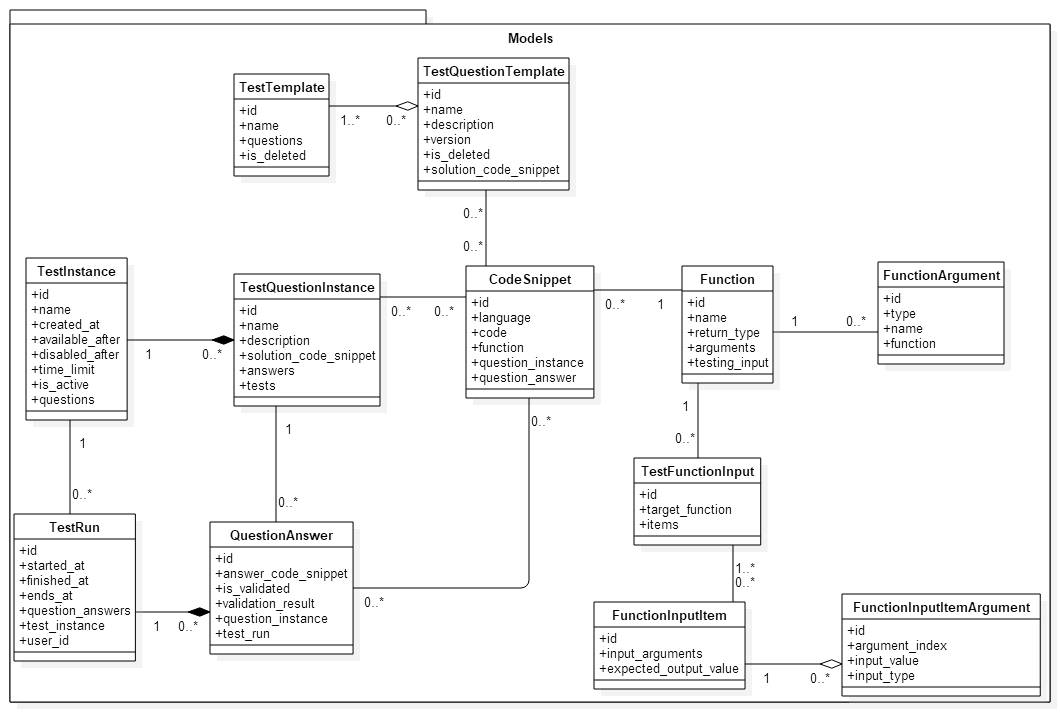
\includegraphics[width=\textwidth]{ClassDiagram_Models}
\end{document}
